\documentclass[../thesis.tex]{subfiles}
\begin{document}
\chapter{Modeling Out-Coupling} \label{sec:out_coupling}

The out-coupling efficiency, \oc is the efficiency of generated photons within an OLED device to exit the device in the forward viewing direction.
Typically, \oc is the limiting component of \eqe, and ranges from 20-30\%.
It is therefore important to understand this quantity and it's dependence on the device geometry.
It is not possible to physically measure this quantity, but extensive modeling has been done to calculate it's value.\supercite{Meerheim2010,Furno2010,Furno2012,Neyts1998}
This chapter will outline the theory that goes into modeling \oc, then proceed into applications for using the model output.

\section{Theory}

Code used for implementation of this theory is provided in Appendix \ref{sec:outCoupling_code}
The implemented model is based off of the models developed in \textcite{Furno2010} and \textcite{Neyts1998}.

A dipole in a planar layer stack can radiate power in any direction.
If we assume the in plane dimensions to be infinite, this system will be radiatively symmetric, and directions can be represented in terms of a unit normalized in-plane wave vector, $u$.
The total power radiated by such a dipole can be expressed as 

\begin{equation}
F=\int_0^\infty K(u)du.
\end{equation}

Here, $F$ is the total radiated power, and $K$ is the power density per unit $du$.
It should be noted that propagating waves are represented by $0\le u\le 1$.
However, $u>1$ represent evanescent wave modes.
In this model, there will be a critical value of $u=u_c$ that will allow light to escape into the substrate in the forward direction.
This power fraction radiated into the substrate can be expressed as

\begin{equation}
\oc=\frac{\int_0^{u_c} K(u)du}{\int_0^\infty K(u)du}.
\label{eqn:out_oc_simple}
\end{equation}

Different polarizations and orientations have different reflection conditions, so must be treated separately.
An emitting dipole in a thin film layer stack can be considered as a superposition of a horizontal ($h$) dipole, oriented perpendicular to the planar system, and vertical ($v$) dipole, oriented within the plane.  
These different orientations can be summed as

\begin{figure}[ht]
\centering
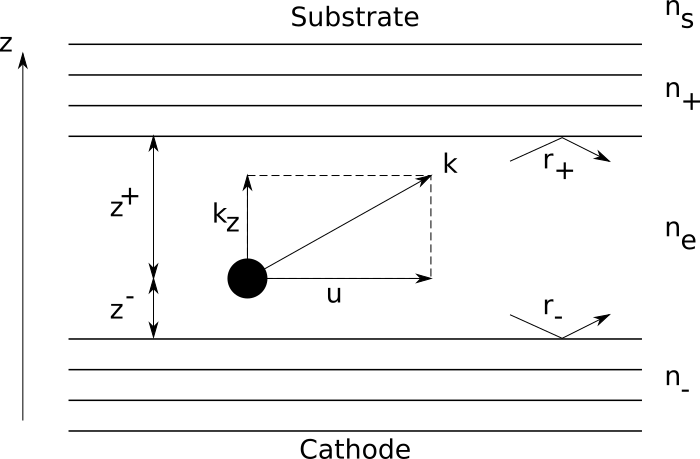
\includegraphics[width=.7\textwidth]{outCoupling/diagram}
\caption{Representation of model quantities.  The positive $z$ axis is shown, along with the wave vector, $k$, the normalized in-plane wave vector, $u$, and the out of plane wave vector, $k_z$.  The positive and negative reflection directions, $r_+$ and $r_-$, respectively.  $n_e$ and $n_s$ are the emitter and substrate indices of refraction, as well as the positive and negative layer stack indices.  $z_+$ and $z_-$ are the distances to the next interface of the emissive layer.}
\label{fig:out_diagram}
\end{figure}

\begin{equation}
K=\frac{1}{3}K_{TM_v}+\frac{2}{3}(K_{TM_h}+K_{TE_h}.
\end{equation}

Where $TM$ represents the transverse magnetic modes and $TE$ is the transverse electric modes.
The power density for these different modes can calculated as

\begin{eqnarray}
K_{TM_v}&=\frac{3}{2}Re\left[\frac{u^3}{\sqrt{1-u^2}}\frac{(1+a_{TM}^+)(1+a_{TM}^-)}{1-a_{TM}}\right] \\
K_{TM_h}&=\frac{3}{4}Re\left[\frac{u}{\sqrt{1-u^2}}\frac{(1-a_{TM}^+)(1-a_{TM}^-)}{1-a_{TM}}\right] \\
K_{TE_h}&=\frac{3}{4}Re\left[u\sqrt{1-u^2}\frac{(1+a_{TE}^+)(1+a_{TE}^-)}{1-a_{TE}}\right] 
\end{eqnarray}

Here $Re$ is the real component of the enclosed quantity. 
Additionally, $a_{TM,TE}^{+,-}$ can be calculated as 

\begin{eqnarray}
a_{TM,TE}^+ &= r_{TM,TE}^+ exp(2jk_{z,e}z^+) \\
a_{TM,TE}^- &= r_{TM,TE}^- exp(2jk_{z,e}z^-)
\end{eqnarray}

\begin{figure}[ht]
\centering
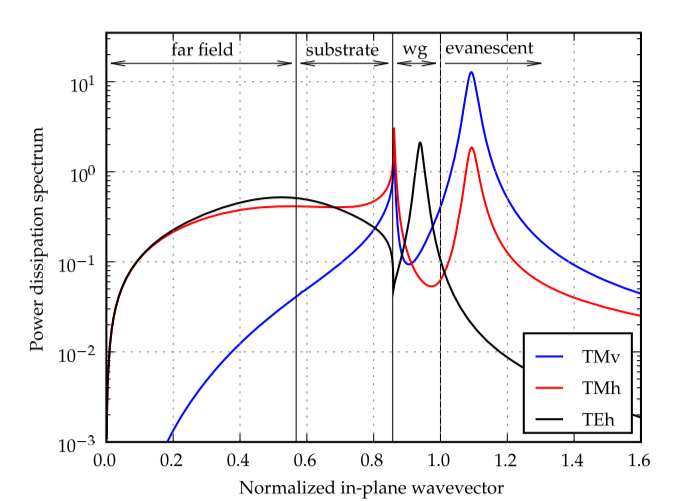
\includegraphics[width=.7\textwidth]{outCoupling/power_density}
\caption{Power Density as a function of $u$ for all three polarizations and orientations. Image taken from \textcite{Furno2010}.}
\label{fig:out_power_density}
\end{figure}

Here, $r$ is the reflection coefficient for waves traveling in the specified direction, with $+$ oriented from the EML towards the cathode, $k_{z,e}$ is the out of plane component of the photon wave vector in the emitting material, and $j=\sqrt{-1}$.
The distance of the dipole from interface is represented as $z^{+,-}$.
These quantities can be seen schematically in Figure \ref{fig:out_diagram}.
The reflection coefficients $r$ can be calculated for arbitrary wave stacks using the transfer matrix model.\supercite{Pettersson1999}
These power densities are used to calculate the total radiated power distribution, shown in Figure \ref{fig:out_power_density}.
In this figure, the loss modes division of $u$ is done using a simple Snell's law calculation.
For coupling into the far field, $u<n_0(\lambda)/n_e(\lambda)$.
For coupling into the substrate, $u<n_s(\lambda)/n_e(\lambda)$.
If $u>1$, this indicates an evanescent mode, with the large peak resulting from the cathode surface plasmon.
The unaccounted for range in $u$ is waveguided in the layer stack.

\subsection{Far Field}

The total radiated power density, $K(u,\lambda)$, is useful for calculating where losses occur within the layer stack.  
However, for far field transmission and the calculation of \oc, a slight modification is needed.
For calculated out-coupled power, the power radiated into the substrate is calculated separately then the substrate transmission is calculated assuming an incoherent material.
The component powers radiated into the substrate is calculated as

\begin{eqnarray}
K_{TM_v}^\prime &= \frac{3}{8}\frac{u^2}{\sqrt{1-u^2}}\frac{\left|1+a_{TM}^-\right|^2}{\left|1-a_{TM}\right|^2}T_{TM}^+ \\
K_{TM_h}^\prime &= \frac{3}{16}\sqrt{1-u^2}\frac{\left|1-a_{TM}^-\right|^2}{\left|1-a_{TM}\right|^2}T_{TM}^+ \\
K_{TE_h}^\prime &= \frac{3}{16}\frac{1}{\sqrt{1-u^2}}\frac{\left|1+a_{TE}^-\right|^2}{\left|1-a_{TE}\right|^2}T_{TE}^+
\end{eqnarray}

and can be summed as before with

\begin{equation}
K^\prime=\frac{1}{3}K^\prime_{TM_v}+\frac{2}{3}(K^\prime_{TM_h}+K^\prime_{TE_h}.
\end{equation}

The factors $T_{TM,TE}^+$ are

\begin{equation}
T_X^+ = |t_{X}^+|^2\frac{n_s}{n_e}\frac{k_{z,s}}{k_{z,e}}
\end{equation}

with $t_{TM,TE}^+$ being the transmission coefficient from transfer matrix calculations, $n_s$ and $n_e$ being the optical constants for the substrate and emissive layer respectively, and $k_z$ is the out of plane wave vector component.
The power radiated out of the substrate can then be calculated with

\begin{equation}
K_{out}=K_{out}^\prime\frac{T_{s,o}}{1-R_{s,o}R_c}
\end{equation}

The total out-coupled power can then be integrated using

\begin{equation}
U(\lambda)=\int_0^{u_{crit}(\lambda)} K_{out}(\lambda,u)du^2
\end{equation}

with the critical dipole orientation obtained from Snell's law by $u_{crit}(\lambda)=n_0(\lambda)/n_e(\lambda)$.
Thus, the efficiency of generated photons can be calculated as

\begin{equation}
\oc=\frac{U(\lambda)}{F(\lambda_)}
\end{equation}

This can be thought of as an integration of the far field portion of Figure \ref{fig:out_power_density} compared to the integration of the whole, with a modification for the transmission through the incoherent substrate.

These calculations allow direct calculation of \oc for a single dipole location and emitter wavelength.
To be accurate for devices, a weighted average of these calculations must be done over the spectral features of the emitter, as well as weighting for the exciton distribution of the recombination zone within the device.



\section{Applications}

\subsection{Gradient EML Recombination Profile Dependence}

Out-coupling efficiency can be an important consideration when designing a high efficiency device.
Even if operating at 100\% internal quantum efficiency, a low \oc can lead to poor device performance.\supercite{Baldo1998a}
For extremely wide recombination zone profiles in devices, there can be a significant change in \oc throughout the device, potentially negating the benefits of the wide recombination zone.
A prime candidate for \oc investigation is the gradient EML (GEML) device, since the RZ can potentially span the majority of the device thickness.\supercite{Erickson2014}

\begin{figure}[ht]
\centering
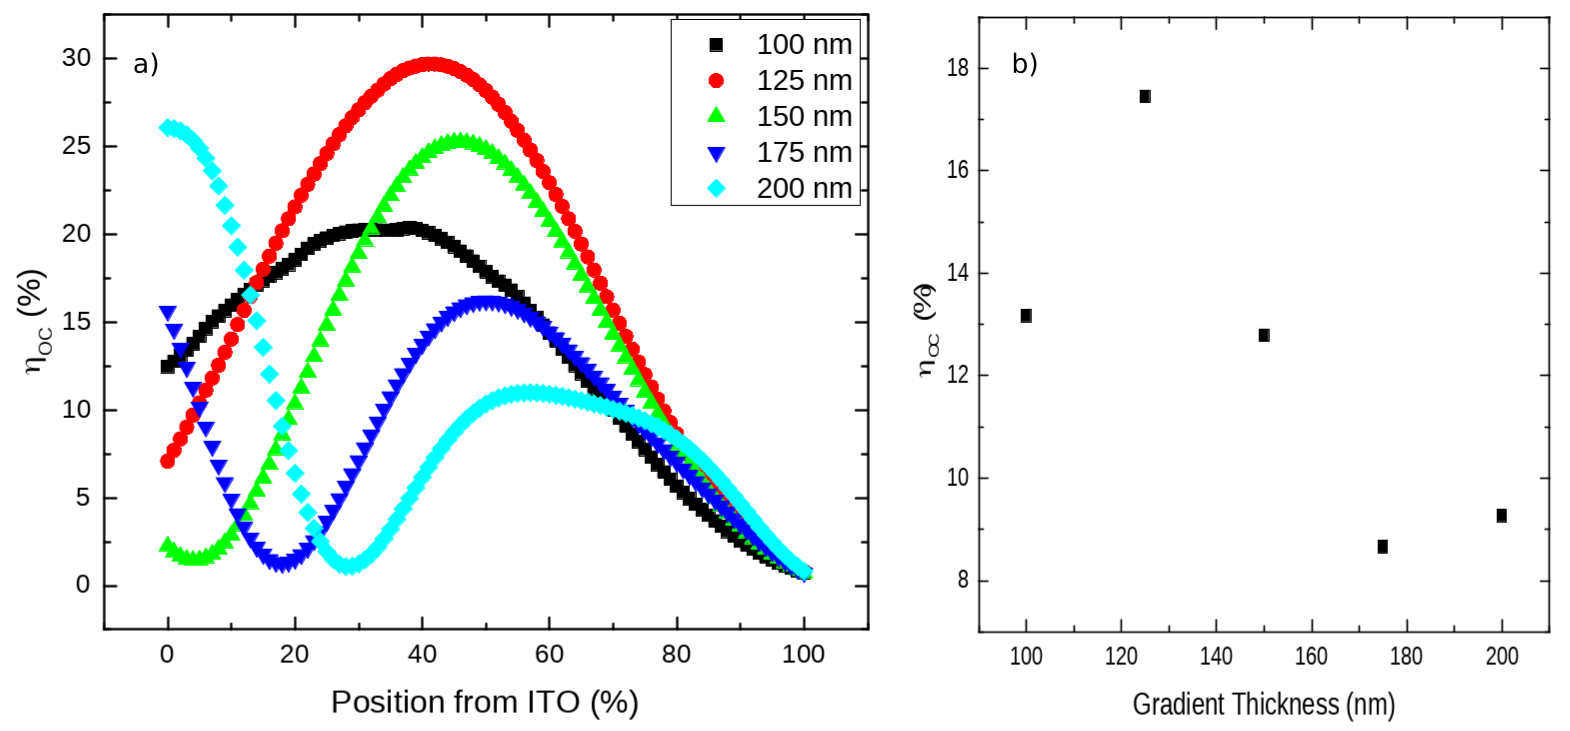
\includegraphics[width=.7\textwidth]{outCoupling/gradient_oc_spatial}
\caption{(a) \oc as a function of normalized device thickness.  (b) The non weighted average of the left panel as a function of gradient thickness.}
\label{fig:gradient_spatial}
\end{figure}

A GEML device consisting of TCTA as an HTL and BPhen as an ETL with 5\% doping of \irppy throughout was investigated.
These device uses a 1:1 gradient profile, meaning that a ramp in the rate of TCTA from 4 to 0 \r{A}/s and BPhen ramps from 0 to 4 \r{A}/s in the same time period with the rate of \irppy held constant.
This results in a 50:50 blend of the HTL and ETL at the midpoint of the device.
The spatial dependence of \oc can be seen in Figure \ref{fig:gradient_spatial}a at $\lambda=512$ nm.

Some common features of \oc profiles should be discussed here.
First off, notice that a near zero boundary condition is observed as the emission dipole nears the cathode interface at 100\% on these profiles.
This is a common feature of \oc profiles in devices and is due to increased coupling to the surface plasmon mode of the cathode.
In organic layer stacks, little change in the index of refraction is seen throughout the stack, and devices often behave similar to a single organic layer.
Going through thick layer stacks, a cyclical peaking of \oc is seen as can be seen in the 175 and 200 nm simulations.
The periodicity of this cycling is a function of wavelength.
Though difficult to see on this normalized axis, for green light, the first peak of this cycle is typically around 40 nm from the cathode.
Most devices are on the order of 100 nm thick, and optimize around the first peak, resulting in ETL thicknesses around 30-40 nm, positioning the EML in this peak.

In Figure \ref{fig:gradient_spatial}b, the non-weighted average of \oc as a function of gradient thickness is shown.  
To be representative of a device, the spatial \oc should be weighted by the RZ profile, but since GEML devices show very broad RZs, this can be a good indicator of device behavior.
It is of note that a significant roll-off in \oc is seen with increasing gradient thickness.  
This is an important design rule, which we noted in Chapter \ref{sec:unified}, for increasing gradient thickness.
Gradients offer a unique ability to distribute the exciton population throughout a device, and were predicted to improve roll-off behavior due to a reduction in bimolecular quenching.
However, as shown by this calculation, the reduction in roll-off is in direct competition with a reduction in peak efficiency due to \oc.
This puts a limit on the amount exciton distribution that is useful for devices.

\begin{wrapfigure}{r}{.5\textwidth}
\centering
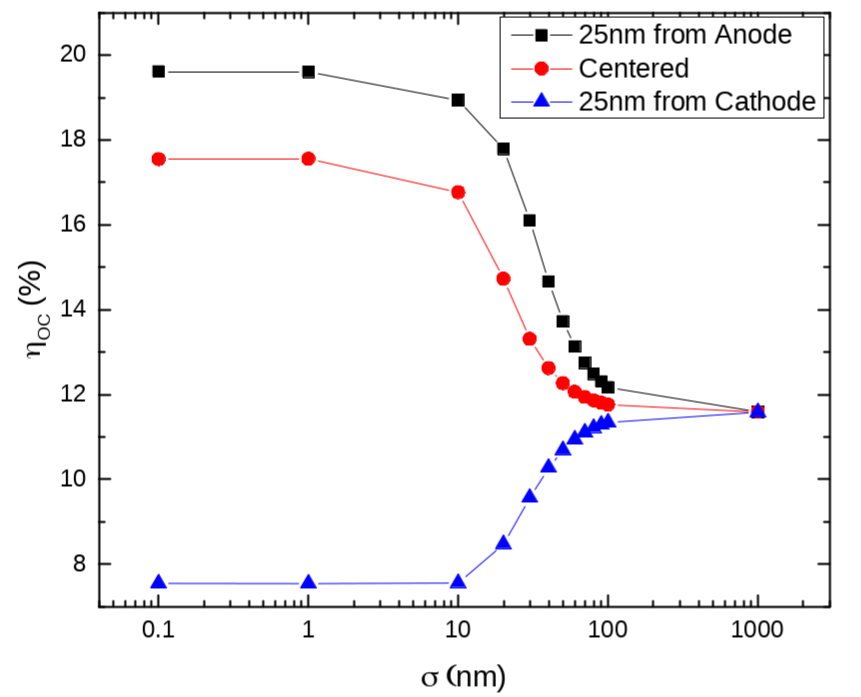
\includegraphics[width=.48\textwidth]{outCoupling/gradient_rz}
\caption{Average \oc for a 100 nm GEML device, weighted to Gaussian recombination zones centered at 25, 50, and 75 nm as a function of the Gaussian width.}
\label{fig:gradient_rz}
\end{wrapfigure}

The spatial profile of the exciton density is also important in calculating of \oc for a device.
GEML devices have broad, featureless RZ profiles, which for the purposes of this modeling, we will assume are Gaussian.\supercite{Erickson2014}.
Figure \ref{fig:gradient_rz} captures dependence of average \oc on the peak position and width of the recombination zone profile.
Three center wavelengths for the RZ profile are shown as a function of the Gaussian width.
The spatial dependence of \oc is shown as the black curve in Figure \ref{fig:gradient_spatial}a.
In Figure \ref{fig:gradient_rz}, the RZ profiles centered at 25 and 50 take advantage of the broad peak in \oc peaked at 35 nm, with the RZ centered at 50 nm showing a closer alignment and thus higher average \oc at sharp RZ profiles near $\sigma=0$.  
The RZ profile centered at 75 nm is too near the cathode and shows a significantly reduced efficiency.
As the RZ profiles broaden, we approach the unweighted behavior, seen as $\lim_{\sigma\to\infty} \oc(\sigma)$.
Again, it is interesting to note that there is a limit in most devices at which broadening the RZ could be detrimental to device behavior due to a reduction in \oc.


\subsection{Exciton Formation Efficiency Extraction}

In Chapter \ref{sec:unified}, a method for extracting the exciton formation efficiency using a model for the transient and steady-state electrical regime was discussed.
In Equation \ref{eqn:eqeReform}, \oc is needed to normalize the resulting modeled behavior for the internal quantum efficiency $\eta_{IQE}$.  
Since a mean field approximation model is being used for this approach, only the average \oc is needed.
However, the recombination zone profile of this device is not known.  
Luckily, only a 10 nm EML is used, and there is minimal change in the \oc as a function of thickness, resulting in reduced error.

\subsection{Recombination Zone Measurement}

\begin{wrapfigure}{r}{.5\textwidth}
\centering
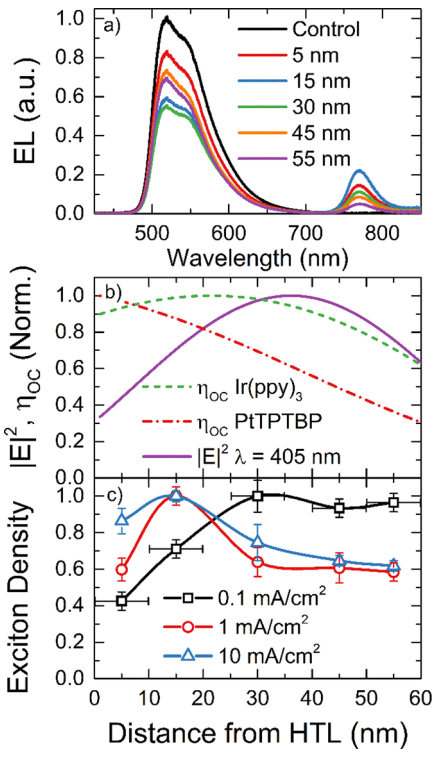
\includegraphics[width=.48\textwidth]{outCoupling/meml_rz}
\caption{(a) Raw electroluminescence spectra of devices with PtTPTBP sensitizer. (b) simulated electric field profile and out-coupling factors at 512 nm and 770 nm. (c) Out-coupling corrected RZ profile. Reproduced from \textcite{Bangsund2018}.}
\label{fig:out_meml_rz}
\end{wrapfigure}

The calculation of the spatial distribution of out-coupling has also been useful for extracting the RZ profile of devices.\supercite{Bangsund2018}
One technique for measuring the recombination zone is to use an emissive sensitizer, that emits spectrally separated from the target emitter, as discussed in Chapter \ref{sec:rz_measurement}.
In this case, we used PtTPTBP ($\lambda_{max}=770 nm$) as a sensitizer for \irppy ($\lambda_{max}=512 nm$), with spectra shown in Figure \ref{fig:out_meml_rz}a.
The simulated \oc, spectrally weighted for the emission of these two emitters is presented in Figure \ref{fig:out_meml_rz}b.
Note the significantly different shape, a result of the significantly longer wavelength of PtTPTBP moving the peak in \oc further from the cathode.
For calculating the RZ shape, without accounting for \oc, one would simply plot the intensity of the 770 nm peak as a function of emitter position.
In Figure \ref{fig:out_meml_rz}a, we can see that this would result in a significant drop off in the RZ intensity as the ETL side interface is approached.
However, from the calculation of \oc, we see that the efficiency is going down in this region.  
The corrected RZ profile is shown in Figure \ref{fig:out_meml_rz}c, and the actual shape can be seen, with a flat recombination zone profile in this region.
This correction for \oc is easy in this method of recombination zone measurement due to the clearly defined emitter position for PtTPTBP.

An alternative approach to measuring the recombination zone is in using a quenching sensitizer which does not emit light.\supercite{Erickson2014}
In this technique, a reduction in the \irppy peak is observed, which corresponds to RZ intensity at that point in space.
The remaining intensity is a function of both the RZ profile and \oc.
Since we are trying to measure the RZ, we cannot use it to correct the data.
This causes a problem for trying to correct the quenching measurement data.
This is somewhat minimized by still seeing emission from a majority of the EML, averaging out the loss, but still presents a problem.

\subsection{PL Accuracy During Decoupled Lifetime Testing}

When decoupling lifetime as discussed in Chapter \ref{sec:integrated_lifetime}, it is important that the EL and PL signals originate from the same position within the device.
This can be assessed by comparing the electric field profile within the device with the measured RZ profile.\supercite{Bangsund2018}
If these are perfectly overlapped, there is no need to consider \oc, but that is likely not the absolute case.
In a more general consideration, The electric field and RZ profiles must be considered for their overlap with the \oc profile.
Analysis of this error is assessed for a particular device system in the Supplementary Material for \textcite{Bangsund2018}, but is found to be $<5\%$ for wide recombination zone devices where strong overlap between these quantities is observed.

During lifetime, an additional out-coupling discrepancy is seen between the EL and PL measurement due to changes in the RZ position as a function of degradation.
If charge transport is degrading, it is very likely that the RZ is moving as the device degrades, though is very difficult to characterize.
If this occurs, the accuracy of the PL measurement changes as a function of degradation due to the overlap of the region probed during EL and PL changing.
Again, investigation of a specific device is discussed in \textcite{Bangsund2018}, and is found to increase in importance as the RZ narrows.


\section{Conclusion}

This section discussed the theory and application of an out-coupling efficiency (\oc) model developed for use with our group.
The careful consideration of \oc is essential to any optical investigation of devices due to the highly variant spatial dependence.
This model has been used for calculations in the steady state behavior as well as lifetime applications.
For lifetimes, broad recombination zones are found to minimize the influence of \oc on the measurements.





\ifcsdef{mainfile}{}{\printbibliography}
\end{document}
